\section{Formalisation in Type Theory}
\paragraph{} Let us recall the two components of the formalisation: 1) translating any
regular expressions to a DFA and 2) proving the correctness of the
translation. 

\paragraph{} In part 1), the translation was divided into the following steps. First, we
followed Thompson's construction algorithm to convert any regular expressions to an
\(\epsilon\)-NFA. Then we removed all the \(\epsilon\)-transitions in
the \(\epsilon\)-NFA by computing the \(\epsilon\)-closure for every states. After that, we used powerset
construction to create a DFA. Finally, we removed all the unreachable
states and then used quotient construction to obtain the minimised
DFA. 

\paragraph{} In part 2), the correctness proos of the above
translation were also separated into different steps according to part
1). For each of the translation steps in part 1), we proved
that the language accepted by the input is equal to the language
accepted by its translated output. i.e. \(L(regex) =
L(translated\ \epsilon\)-NFA\() = L(translated\) DFA\() =
L(translated\) MDFA\()\). 

\paragraph{} In the following parts, we will walk through the formalisation of
each of the above steps together with their correctness proofs. Note
that all the definitions, theorems, lemmas and proofs wriiten in below
are adapted to the formalisation in Agda. Now, before we go into
regular expressions and automata, we first need to have a
representation of subsets and languages as they are fundamental
elements in the theory. 

\subsection{Subsets and Decidable Subsets}

\paragraph{Definition 1.1} Suppose \(A\) is a set, in Type Theory, its
subsets are represented as a unary function on
\(A\), i.e. \(Subset\ A = A \to Set\). 

\paragraph{} When declaring a subset in Agda, we can write \(SubA =
\lambda\ a \to\ ?\), the \(?\) here defines the
condition for \(a\) to be included in \(SubA\). This construction is
very similar to set comprehension. For example, the subset 
\(\{a\ | \ a \in A,\ P(a)\}\) corresponds to \(\lambda\ a \to P\
a\). Subset is also a unary predicate of \(A\); therefore, the decidability of it will remain
unknown until it is proved. 

\paragraph{Definition 1.2} The other representation of subset is \(DecSubset\ A = A \to
Bool\). Unlike \(Subset\), its decidability is ensured by its
definition. 

\paragraph{} The two definitions have different purposes. \(Subset\) is used to represent \(Language\) because not every
language is decidable. For other parts 
such as a subset of states in an automaton, \(DecSubset\) is used
as the decidability is assumed in the definition. The two definitions
are defined in Subset.agda and Subset/DecidableSubset.agda
respectively as stated at the top. Operators such as membership (\(\in\)), subset
(\(\subseteq\)), superset (\(\supseteq\)) and equality (\(=\)) can
also be found in the two files. 

\subsubsection{Operations on Subsets}
\paragraph{}

\subsubsection{Operations on Decidable Subsets}
\paragraph{}

\paragraph{} Now, by using the representation of subset, we can define languages, regular expressions and finite
automata. 

\subsection{Languages}

\paragraph{} Suppose we have a set of alphabets \(\Sigma\); in Type Theory, it
can be represented as a data type, i.e. \(\Sigma : Set\). Notice that the decidable equality of
\(\Sigma\) is assumed. In Agda, they are passed to every modules as
parameters \((\Sigma : Set)\) \((dec : DecEq\ \Sigma)\). 

\paragraph{Definition 2.1} We first define \(\Sigma^*\) as the set of all
strings over \(\Sigma\). In our approach, it was expressed as a list of
\(\Sigma\), i.e. \(\Sigma^* = List\ \Sigma\). 

\paragraph{} For example, (\(A :: g ::
d :: a :: []\)) represents the string 'Agda' and the empty list \([]\)
represents the empty string \(\epsilon\). In this way, we can pattern
match on the input string in order to get the first
input alphabet and to run a transition from a particular state to another state. 

\paragraph{Definition 2.2} A language is a subset of 
\(\Sigma^*\); in Type Theory, \(Language = Subset\ \Sigma^*\). 
Notice that \(Subset\) instead of \(DecSubset\) is used because not every language is decidable. 

\subsubsection{Operations on Languages}

\paragraph{Definition 2.3} If \(L_1\) and \(L_2\) are languages, then
the union of the two languages \(L_1\cup L_2\) is defined as \(\{w\
|\  w \in L_1\ \vee \ w \in
L_2\}\). In Type Theory, we define it as \(L_1 \cup L_2 = \lambda\ w
\to w \in L_1\ \uplus\ w \in L_2\).

\paragraph{Definition 2.4} If \(L_1\) and \(L_2\) are languages, then
the concatenation of the two languages \(L_1\bullet L_2\) is defined
as \(\{w\  |\  \exists u\in L_1.\ \exists v\in L_2.\ w = uv\}\). In
Type Theory, we define it as \(L_1\bullet L_2 = \lambda\ w \to \exists[
u \in \Sigma^* ]\ \exists[ v \in \Sigma^* ] ( u \in L_1 \times v \in L_2 \times w \equiv u\ ++\ v ) \).

\paragraph{Definition 2.5} If \(L\) is a language, then the closure of
L, \(L\ast\) is defined as \( \bigcup_{n \in N} L^n \) where
\( L^n = L\bullet L^{n - 1} \) and \(L^0 = \{\epsilon\}\). In Type
Theory, we have \(L\ \star = \lambda w \to \exists [ n \in \mathbb{N}
]( w \in L\ \)\^\ \(n)\) where the function \_\^ \_ is defined
recursively as: 
\begin{lstlisting}[mathescape=true,xleftmargin=.3\textwidth,aboveskip=0pt,belowskip=0pt]
_^_ : Language $\to$ Language $\to$ Language
L ^ zero    = $[\![\epsilon ]\!]$
L ^ (suc n) = L $\bullet$ L ^ n
\end{lstlisting}

\subsection{Regular Languages and Regular Expressions}

\paragraph{Definition 3.1} We define regular languages over
\(\Sigma\) inductively as follow:
\begin{enumerate}[nolistsep]
  \item \(\O\) is a regular language;
  \item \(\{\epsilon\}\) is a regular language;
  \item \(\forall a\in\Sigma.\ \{a\}\) is a regular language;
  \item if \(L_1\) and \(L_2\) are regular languages, then
    \begin{enumerate}[nolistsep]
      \item \(L_1\cup L_2\) is a regular language;
      \item \(L_1\bullet L_2\) is a regular language;
      \item \(L_1\ \star\) is a regular language.
    \end{enumerate}
\end{enumerate}
\vspace{0.7pc}
\begin{lstlisting}[caption=Regular languages,mathescape=true]
data Regular : Language $\to$ Set$_1$ where
  nullL : $\forall$ {L} $\to$ L $\approx$ $\o$ $\to$ Regular L
  empty : $\forall$ {L} $\to$ L $\approx$ $[\![\epsilon ]\!]$ $\to$ Regular L
  singl : $\forall$ {L} $\to$ (a : $\Sigma$) $\to$ L $\approx$ $[\![a]\!]$ $\to$ Regular L
  union : $\forall$ {L} L$_1$ L$_2$ $\to$ Regular L$_1$ $\to$ Regular L$_2$ $\to$ L $\approx$ $L_1\ \cup\ L_2$ $\to$ Regular L
  conca : $\forall$ {L} L$_1$ L$_2$ $\to$ Regular L$_1$ $\to$ Regular L$_2$ $\to$ L $\approx$ $L_1\ \bullet\ L_2$ $\to$ Regular L
  kleen : $\forall$ {L} L$_1$ $\to$ Regular L$_1$ $\to$ L $\approx$ L$_1\ \star$ $\to$ Regular L
\end{lstlisting}

\paragraph{Definition 3.2} Here we define regular expressions
inductively over \(\Sigma\) as follow: 
\begin{enumerate}[nolistsep]
  \item \(\O\) is a regular expression denoting the regular language \(\O\);
  \item \(\epsilon\) is a regular expression denoting the regular language \(\{\epsilon\}\);
  \item \(\forall a\in\Sigma.\ a\) is a regular expression denoting the regular language \(\{a\}\);
  \item if \(e_{1}\) and \(e_{2}\) are regular expressions denoting the regular
    languages \(L_1\) and \(L_2\) respectively, then
    \begin{enumerate}[nolistsep]
      \item \(e_{1}\ |\ e_{2}\) is a regular expressions denoting the
        regular language \(L_1 \cup L_2\);
      \item \(e_{1}\cdot e_{2}\) is a regular expression denoting the
        regular language \(L_1\bullet L_2\);
      \item \(e_{1}^{\ *}\) is a regular expression denoting the regular
        language \(L_1\ \star\).
     \end{enumerate}
\end{enumerate}
%\vspace{1pc}
\paragraph{} The Agda formalisation is separated into two parts, firstly the
definition of regular expressions and secondly the languages denoted by
them.

\begin{lstlisting}[caption=Regular expressions,mathescape=true]
data RegExp : Set where
  $\O$    : RegExp
  $\epsilon$    : RegExp
  $\sigma$    : $\Sigma$ $\to$ RegExp
  _|_ : RegExp $\to$ RegExp $\to$ RegExp
  _$\cdot$_  : RegExp $\to$ RegExp $\to$ RegExp
  _$^*$  : RegExp $\to$ RegExp
\end{lstlisting} 

\begin{lstlisting}[caption=Languages denoted by regular expressions,mathescape=true]
L$^R$ : RegExp $\to$ Language
L$^R$ $\O$   = $\o$
L$^R$ $\epsilon$   = $[\![\epsilon ]\!]$
L$^R$ ($\sigma$ a) = $[\![a]\!]$
L$^R$ (e$_1$ | e$_2$) = L$^R$ e$_1$ $\cup$ L$^R$ e$_2$
L$^R$ (e$_1$ $\cdot$ e$_2$) = L$^R$ e$_1$ $\bullet$ L$^R$ e$_2$
L$^R$ (e$^*$) = (L$^R$ e) $\star$
\end{lstlisting}

\subsection{\(\epsilon\)-Non-deterministic Finite Automata}

\paragraph{} By now, the set of strings we have considered are in the form of
\(List\ \Sigma^*\). However, this definition gives us no way to
extract an \(\epsilon\)-transition from the input string. Therefore, we need to introduce another
representation of the set of strings specifically for this purpose. (For Definition 4.1 and
4.2, please refers to Language.agda)

\paragraph{Definition 4.1} We define \(\Sigma^e\) as the union of
\(\Sigma\) and \(\{\epsilon\}\), i.e. \(\Sigma^e = \Sigma \cup
\{\epsilon\}\). 

\paragraph{} In Agda, this can be expressed by a data type definition:
\begin{lstlisting}[mathescape=true,xleftmargin=.4\textwidth,aboveskip=0pt,belowskip=0pt]
data $\Sigma^e$ : Set where
  $\alpha$ : $\Sigma \to \Sigma^e$
  E : $\Sigma^e$
\end{lstlisting}

\paragraph{Definition 4.2} Now we define \(\Sigma^{e*}\), the set of all strings over
\(\Sigma^e\) in a way similar to \(\Sigma^*\), i.e. \(\Sigma^{e*} =
List\ \Sigma^e\). 

\paragraph{} For example, the string 'Agda' can be
represented by (\(\alpha\ A ::\ \alpha\ g :: E ::\ \alpha\ d :: E ::\ \alpha\
a :: []\)) or (\(E ::\ \alpha\ A :: E :: E ::\ \alpha\ g ::\ \alpha\ d :: E ::\ \alpha\
a :: []\)). We say that these two lists are
\(\epsilon\)-strings of the word 'Agda'. When pattern matching on an \(\epsilon\)-string, we
can know if there is an \(\epsilon\)-transition or not. Other operators and lemmas
regarding \(\epsilon\)-strings such
as \(to\Sigma^*\ :\ \Sigma^{e*} \to \Sigma^*\) can also be found in
Language.agda. 

\paragraph{} Now, let us define \(\epsilon\)-NFA. 

\paragraph{Definition 4.3} An \(\epsilon\)-NFA is a 5-tuple \(M = (Q
,\ \Sigma^e,\ \delta,\ q_0,\ F)\), where
\begin{enumerate}[nolistsep]
  \item \(Q\) is a finite set of states;
  \item \(\Sigma^e\) is the union of \(\Sigma\) and \(\{\epsilon\}\);
  \item \(\delta\) is a mapping from \(Q \times\ \Sigma^e\) to
    \(\mathcal P \left({Q}\right)\) which defines the behaviour of the automata;
  \item \(q_0\) in \(Q\) is the initial state;
  \item \(F \subseteq Q\) is the set of accepting states. 
\end{enumerate}
\vspace{0.7pc}
\begin{lstlisting}[caption=\(\epsilon\)-NFA,mathescape=true]
record $\epsilon \hyphen$NFA : Set$_1$ where
  field
    Q      : Set
    $\delta$       : Q $\to$ $\Sigma^e$ $\to$ DecSubset Q
    q$_0$      : Q
    F      : DecSubset Q
    $\forall$qEq    : $\forall$ q $\to$ q $\in^d$ $\delta$ q E
    Q?     : DecEq Q
    |Q|-1  : $\mathbb{N}$
    It     : Vec Q (suc |Q|-1)
    $\forall$q$\in$It    : (q : Q) $\to$ (q $\in^V$ It)
    unique : Unique It
\end{lstlisting}
%\vspace{1pc}
\paragraph{} The set of alphabets \(\Sigma : Set\) is passed to the file
parameters. Together with \(Q\), \(\delta\),
\(q_0\) and \(F\), these five fields correspond to the 5-tuple
\(\epsilon\)-NFA. \(\forall qEq\) is a proof that any state in \(Q\)
can reach itself by an \(\epsilon\)-transition. \(Q?\) is
the decidable equality of \(Q\). \(|Q|-1\) is the number of states -
1. '\(It\)' is a vector of length \(|Q|\) containing all the
states in \(Q\). \(\forall q\in It\) is a
proof that all states in \(Q\) are also in the vector
'\(It\)'. \(unique\) is a proof that there is no repeating elements in
'\(It\)'. These extra fields are important when computing
\(\epsilon\)-closures, we will look into them again later in more
details.  

\paragraph{} Now, we want to define the set of strings \(\Sigma^*\) accepted by a given
\(\epsilon\)-NFA. However, before we can do this, we have to define
some operations.

\paragraph{Definition 4.4} A configuration is a pair \(Q \times
\Sigma^{e*}\). Notice that the configuration is based on
\(\Sigma^{e*}\) but not \(\Sigma^*\).

\paragraph{Definition 4.5} A move by an \(\epsilon\)-NFA \(N\) is
represented by a binary function \(\vdash\) on configurations. We say
that \((q, aw) \vdash (q' , w)\) for all w in \(\Sigma^{e*}\)
if and only if \(q' \in \delta (q , a)\) where \(a \in \Sigma^e\). 

\begin{lstlisting}[mathescape=true]
  _$\vdash$_ : (Q $\times$ $\Sigma^e$ $\times$ $\Sigma^{e*}$) $\to$ (Q $\times$ $\Sigma^{e*}$) $\to$ Set
  (q , a , w) $\vdash$ (q' , w') = w $\equiv$ w' $\times$ q' $\in^d$ $\delta$ q a
\end{lstlisting}

\paragraph{Definition 4.6} We say that \(C \vdash^0 C'\) if and only
if \(C = C'\). We say that \(C_0 \vdash^k C_k\) for any \(k \geq 1\) if and only if there exists a chain of
configurations \(C_1, C_2, ..., C_{k-1}\) such that \(C_i \vdash
C_{i+1}\) for all \(0 \leq i \leq k\). 

\begin{lstlisting}[mathescape=true]
  _$\vdash^k$_-_ : (Q $\times$ $\Sigma^{e*}$) $\to$ $\mathbb{N}$ $\to$ (Q $\times$ $\Sigma^{e*}$) $\to$ Set
  (q , w$^e$) $\vdash^k$ zero  - (q' , w$^e$')
    = q $\equiv$ q' $\times$ w$^e$ $\equiv$ w$^e$'
  (q , w$^e$) $\vdash^k$ suc n - (q' , w$^e$') 
    = $\exists$[ p $\in$ Q ] $\exists$[ a$^e$ $\in$ $\Sigma^e$ ] $\exists$[ u$^e$ $\in$ $\Sigma^{e*}$ ]
      (w$^e$ $\equiv$ a$^e$ :: u$^e$ $\times$ (q , a$^e$ , u$^e$) $\vdash$ (p , u$^e$) $\times$ (p , u$^e$) $\vdash^k$ n - (q' , w$^e$'))
\end{lstlisting}

\paragraph{Definition 4.7} We say that \(C \vdash^* C'\) if and only
if there exists a number of chains \(n\) such that \(C \vdash^n C'\). 

\begin{lstlisting}[mathescape=true]
  _$\vdash^*$_ : (Q $\times$ $\Sigma^{e*}$) $\to$ (Q $\times$ $\Sigma^{e*}$) $\to$ Set
  (q , w$^e$) $\vdash^*$ (q' , w$^e$') = $\exists$[ n $\in$ $\mathbb{N}$ ] (q , w$^e$) $\vdash^k$ n - (q' , w$^e$')
\end{lstlisting}

\paragraph{Definition 4.8} For any string \(w\), it is accepted by an \(\epsilon\)-NFA \(N\)
if and only if there exists a chain of configurations from \(q_0 ,
w^e)\) to \(q , \epsilon\) where \(w^e\) is an \(\epsilon\)-string of \(w\) and \(q \in
F\). 

\paragraph{Definition 4.9} The language accepted by an
\(\epsilon\)-NFA is given by the set \(\{\ w\ |\ \exists w^e\in
\Sigma^{e*}.\ w = to\Sigma^*(w^e) \wedge \exists q\in F.\ (q_0\ ,\
w^e) \vdash^* (q\ ,\ \epsilon)\ \}\). 

\begin{lstlisting}[mathescape=true]
  L$^{eN}$ : $\epsilon \hyphen$NFA $\to$ Language
  L$^{eN}$ nfa = $\lambda$ w $\to$ 
            $\exists$[ w$^e$ $\in$ $\Sigma^{e*}$ ] (w $\equiv$ $to\Sigma^*$ w$^e$ $\times$ ($\exists$[ q $\in$ Q ] (q $\in^d$ F $\times$ (q$_0$ , w$^e$) $\vdash^*$ (q , []))))
\end{lstlisting} 
%\vspace{1pc}
\paragraph{} Now that we have the definition of regular expressions and
\(\epsilon\)-NFA, we can formulate the translation using Thompson's Construction.

\subsection{Thompson's Construction}

\paragraph{Definition 5.1} The translation for any regular expressions
to an \(\epsilon\)-NFA is defined inductively as follow:
\begin{enumerate}[nolistsep]
  \item for \(\O\), we have \(M = (\{init\},\ \Sigma^e,\ \delta,\
    init,\ \O)\) and graphically \begin{center}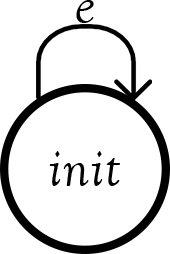
\includegraphics{null}\end{center}
  \item for \(\epsilon\), we have \(M = (\{init\},\ \Sigma^e,\
    \delta,\ init,\ \{init\})\) and graphically \begin{center}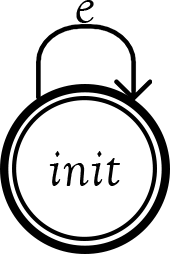
\includegraphics{epsilon}\end{center}
  \item for \(a\), we have \(M = (\{init, accept\},\ \Sigma^e,\
    \delta,\ init,\ \{accept\})\) and graphically \begin{center}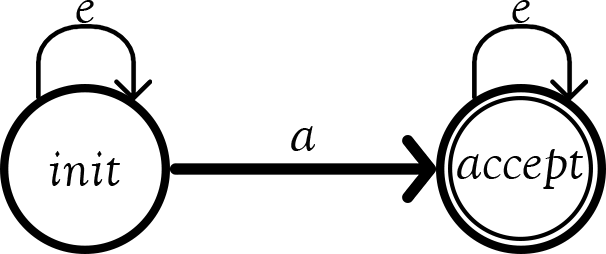
\includegraphics{singleton}\end{center}
  \item if \(N_1 = (Q_1,\ \delta_1,\ q_{01},\ F_1)\) and \(N_2 =
    (Q_2,\ \delta_2,\ q_{02},\ F_2)\) are \(\epsilon\)-NFAs translated from the
    regular expressions \(e_1\) and \(e_2\) respectively, then
    \begin{enumerate}[nolistsep]
      \item for \((e_1\ |\ e_2)\), we have \(M = (\{init\} \cup Q_1
        \cup Q_2,\ \Sigma^e,\ \delta,\ init,\ F_1 \cup F_2)\) and
        graphically \begin{center}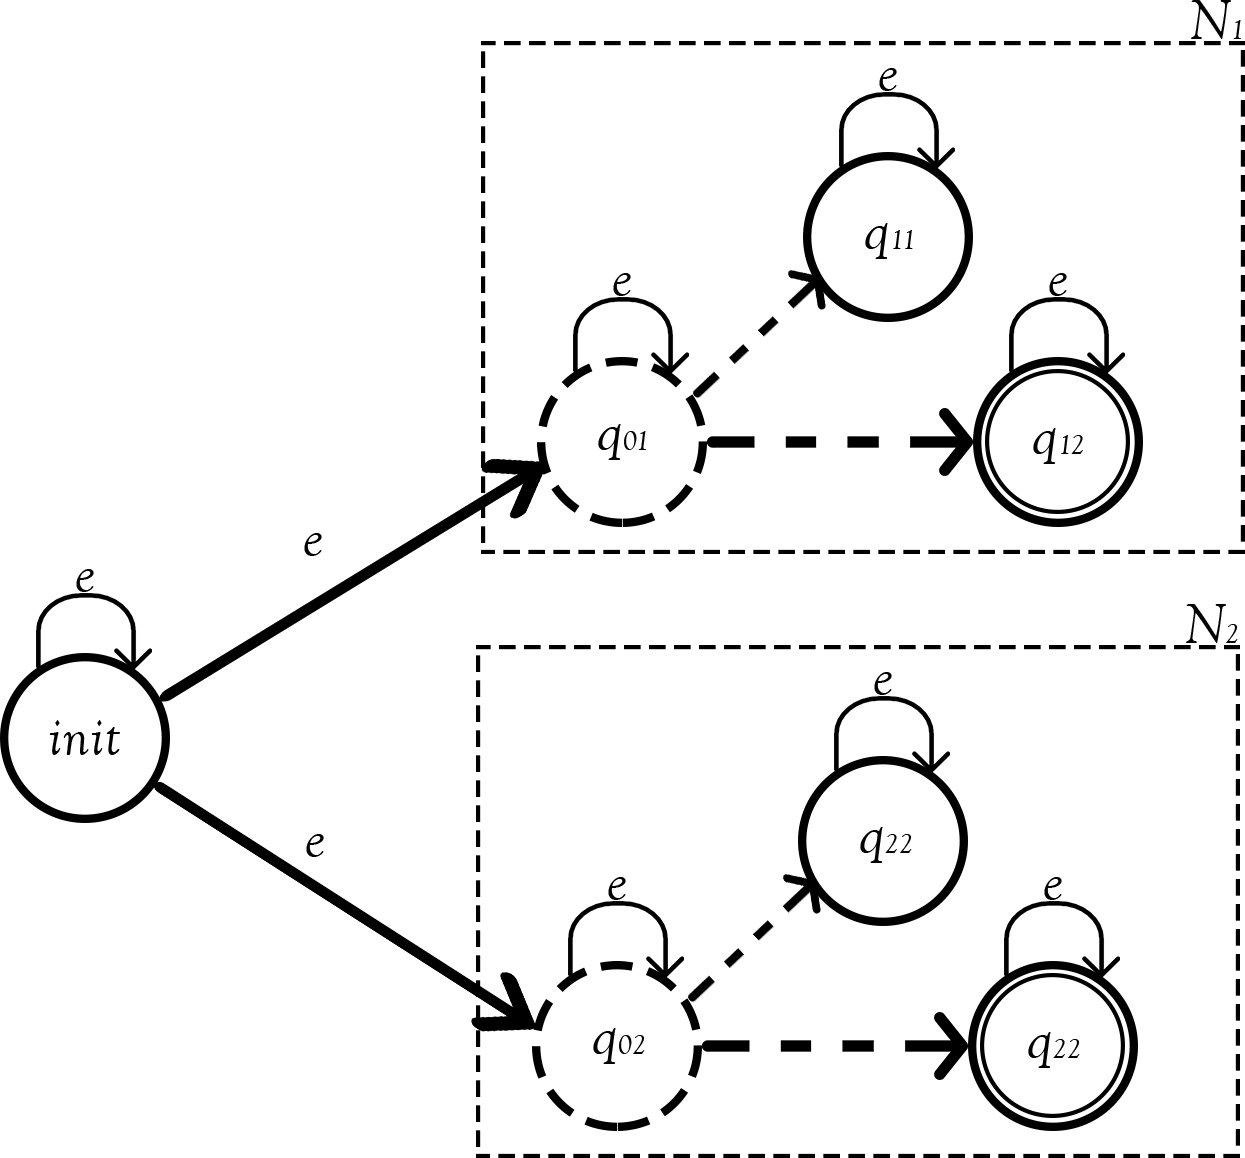
\includegraphics{union}\end{center}
      \item for \(e_1\cdot e_2\), we have \(M = (Q_1 \cup \{mid\}
        \cup Q_2,\ \Sigma^e,\ \delta,\ init,\ F_2)\) and graphically \begin{center}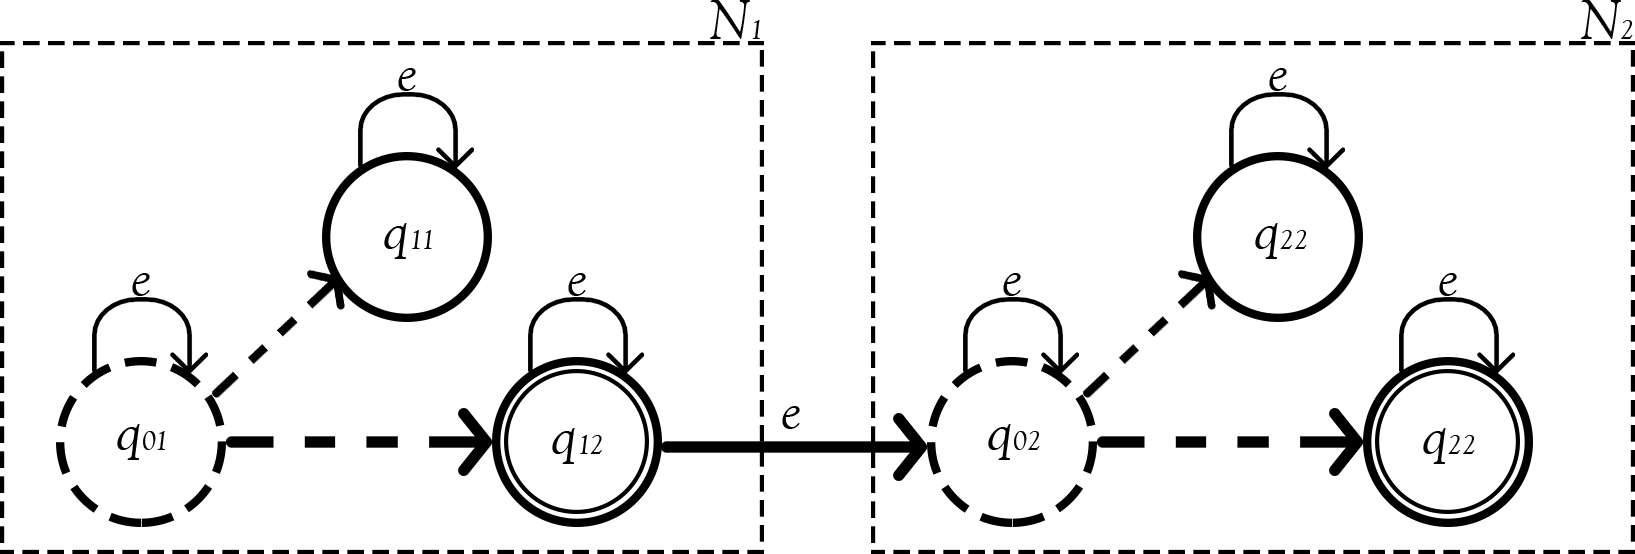
\includegraphics{concat}\end{center}
      \item for \(e_1^{\ *}\), we have \(M = (\{init\} \cup Q_1,\
        \Sigma^e,\ \delta,\ init,\ \{init\} \cup F_1)\) and
        graphically \begin{center}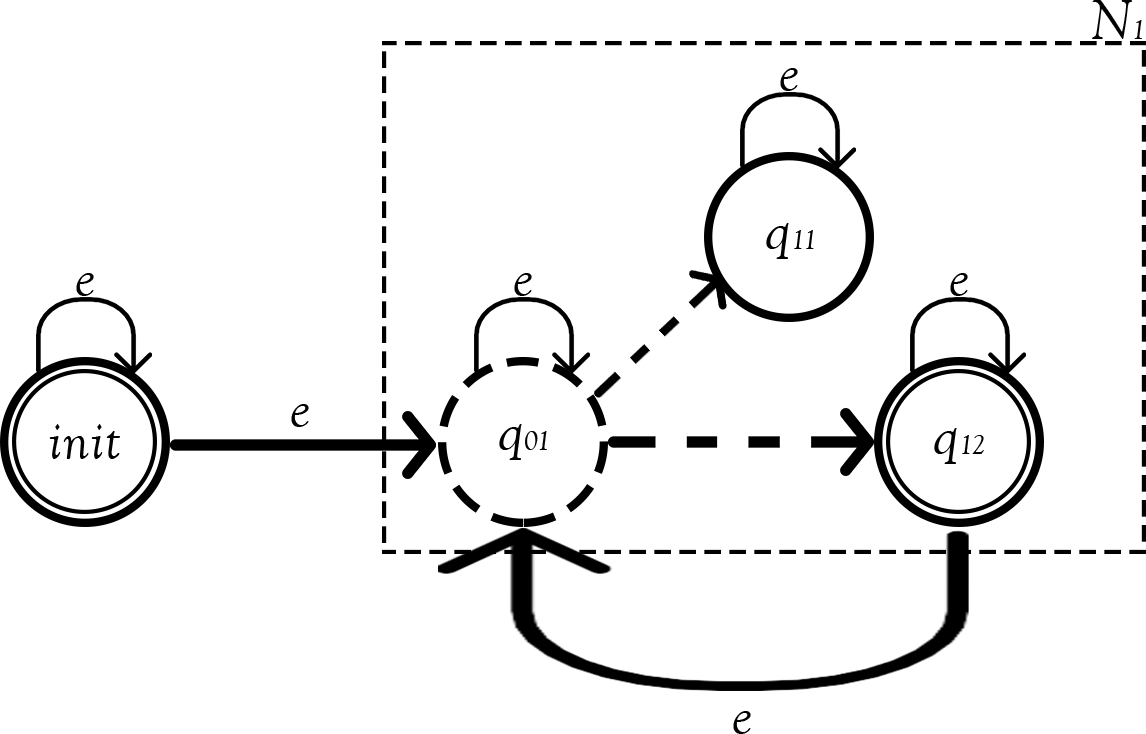
\includegraphics{star}\end{center}
     \end{enumerate}
\end{enumerate}


\paragraph{Theorem 1.1} For any given regular expressions, its accepted
language is equal to the language accepted by its translated
\(\epsilon\)-NFA using Thompson's Construction. i.e. \(L(e) =
L(translted\ \epsilon\)-NFA\()\). 

\paragraph{Proof 1.1} We have to prove that for any regular expressions \(e\), \(L(e) \subseteq
L(translated\ \epsilon\)-\(NFA)\) and \(L(e) \supseteq L(translated\
\epsilon\)-\(NFA)\) by induction on \(e\). 

\subparagraph{Base cases} For \(\O\), \(\epsilon\) and \(a\), by Definition 5.1, it is obvious that the
language accepted by them are equal to the language accepted by their
translated \(\epsilon\)-NFA. 

\subparagraph{Induction hypothesis} For any regular expressions
\(e_1\) and \(e_2\), let \(N_1 =
(Q_1,\ \delta_1,\ q_{01},\ F_1)\) and \(N_2 = (Q_2,\ \delta_2,\
q_{02},\ F_2)\) be their translated \(\epsilon\)-NFA using Definition
5.1 respectively. Then we assume that \(L(e_1) = L(N_1)\) and \(L(e_2) =
L(N_2)\). 
\\
\par \textbf{Inductive steps}
\par 1) For \((e_1\ |\ e_2)\), let \(M = (Q,\ \delta,\ q_0,\ F) = (\{init\} \cup Q_1 \cup Q_2,\
\delta,\ init,\ F_1 \cup F_2)\) be its translated \(\epsilon\)-NFA
using Definition 5.1. Then for any string \(w\), 

\par 1.1) if \((e_1\ |\ e_2)\) accepts \(w\), by Definition 3.2,
either i) \(e_1\) accepts \(w\) or ii) \(e_2\) accepts \(w\). Assuming case i), then by
induction hypothesis, \(N_1\) also accepts \(w\) which also implies
that there exists a chain \((q_{01} , w^e) \vdash^* (q , \epsilon)\) in \(N_1\) such that
\(w^e\) is an \(\epsilon\)-string of \(w\) and \(q \in F_1\). Now, we can
add an \(\epsilon\)-transition from \(init\) to \(q_{01}\) in \(M\)
such that \((init , \epsilon w^e) \vdash^* (q , \epsilon)\)
because \(q_{01} \in \delta\ init\ \epsilon\). Now, since \(q \in
F_1\) implies that \(q \in F\) and \(\epsilon w^e\)
is also an \(\epsilon\)-string of \(w\); therefore \(w \in L(M)\). The same argument also applies
for the case when \(e_2\) accepts \(w\). Since we have proved that \(w \in L(e_1\ |\ e_2)
\Rightarrow w \in L(M)\); therefore \(L(e_1\ |\ e_2) \subseteq L(M)\)
also follows;

\par 1.2) if \(M\) accepts \(w\), then there must exists a chain \((init , w^e) \vdash^* (q ,
\epsilon)\) in \(M\) such that \(w^e\) is an \(\epsilon\)-string of \(w\) and \(q
\in F\). Since \(q \in F\), therefore \(q \neq init\). By Definition
5.1, there are only two possible ways for \(init\) to reach \(q\), via \(q_{01}\) or ii) 
\(q_{02}\). Assuming case i), then we have \((init , \epsilon^+w_1) \vdash^*
(q_{01} , w_1)\) and \((q_{01} , w_1) \vdash^* (q , \epsilon)\) where \(w^e =
\epsilon^+w_1\) and \(q \in Q_1\). Since we have \(q \in F\) and \(q \in
Q_1\); therefore we have \(q \in F_1\). Also \(w_1\) is also an
\(\epsilon\)-string of \(w\), thus the chain \((q_{01} , w_1) \vdash^* (q , \epsilon)\)
implies that \(w \in L(N_1)\). By induction hypothesis, we have \(w \in L(e_1)\) and thus \(w \in L(e_1\
|\ e_2)\). The same argument also applies for case ii). Since we have
proved that \(w \in
L(M) \Rightarrow w \in L(e_1\ |\ e_2)\); therefore \(L(e_1\ |\ e_2)
\supseteq L(M)\) also follows;

\par 1.3) combining 1.1  and 1.2, we have \(L(e_1\ |\ e_2) = L(M)\). 
\\
\par 2) For \((e_1 \cdot e_2)\), let \(M = (Q,\ \delta,\ q_0,\ F) = (Q_1 \cup \{mid\} \cup Q_2,\ \delta,\ q_{01},\ F_2)\) be its
translated \(\epsilon\)-NFA using Definition 5.1. Then for any string
\(w\), 

\par 2.1) if \((e_1 \cdot e_2)\) accepts \(w\), then by Definition
3.2, there exists a \(u \in L(e_1)\) and a \(v \in L(e_2)\) such that \(w
= uv\). By induction hypothesis, \(u \in L(e_1)\) implies that \(u \in
L(N_1)\) and \(v \in L(e_2)\) implies that \(v \in L(N_2)\). So there
exists a chain: i)\((q_{01} ,
u^e) \vdash^* (q_1 , \epsilon)\) in \(N_1\) where
\(u^e\) is an \(\epsilon\)-string of \(u\) and \(q_1 \in F_1\) and
ii) \((q_{02} , v^e) \vdash^* (q_2 , \epsilon)\) in \(N_2\)
where \(v^e\) is an \(\epsilon\)-string of \(v\) and \(q_2 \in
F_2\). Now we can add an \(\epsilon\)-transition from \(q_1\) to \(mid\) and
from \(mid\) to \(q_{02}\) in order to construct a chain in
\(M\). Since\(q_2
\in F_2\) implies that \(q_2 \in F\) and \(u^ev^e\) is an
\(\epsilon\)-string of \(w\) implies that so is \(u^e\epsilon \epsilon
v^e\); therefore \(w \in L(M)\). Since we have proved that \(w \in
L(e_1 \cdot e_2) \Rightarrow w \in L(M)\), therefore \(L(e_1 \cdot
e_2) \subseteq L(M)\) also follows;

\par 2.2) if \(M\) accepts \(w\), then by Definition 5.1, there must exists
a chain \((init , w^e) \vdash^* (q , \epsilon)\) in \(M\) where
\(w^e\) is an \(\epsilon\)-string of \(w\) and \(q \in F\). Since \(q
\in F\), so \(q\) must also be in \(Q_2\). The only possible way for
\(q_{01}\) to reach \(q\) is to go through \(mid\). This implies that
there exists a \(q_1 \in Q_1\), a \(u^e \in \Sigma^{e*}\) and a \(v^e \in
\Sigma^{e*}\) such that \((q_{01} , u^e\epsilon^+ \epsilon^+ v^e) \vdash^*
(q_1 , \epsilon^+ \epsilon^+ v^e)\), \(q_1 \in F_1\), \((q_{02} , v^e)
\vdash^* (q_2 , \epsilon)\) and \(w^e = u^e\epsilon^+ \epsilon^+
v^e\). Let \(u\) and \(v\) be the strings represented by \(u^e\) and
\(v^e\) respectively, we have \(u \in L(N_1)\) and \(v \in
L(N_2)\). Then, by induction hypothesis, \(u \in L(e_1)\) and \(v \in
L(e_2)\). Since \(w^e\) is an \(\epsilon\)-string of \(w\), so is
\(u^ev^e\) and thus \(w =
uv\). From this, we can deduce that \(w \in L(e_1 \cdot e_2)\). Since
we have proved that \(w \in L(M) \Rightarrow w \in L(e_1 \cdot e_2)\),
therefore \(L(e_1 \cdot e_2) \supseteq L(M)\) also follows;

\par 2.3) combining 2.1 and 2.2, we have \(L(e_1 \cdot e_2) = L(M)\). 
\\
\par 3) For \(e^*\), let \(M = (Q,\ \delta,\ q_0,\ F) = (Q_1 \cup \{mid\} \cup Q_2,\ \delta,\ q_{01},\ F_2)\) be its
translated \(\epsilon\)-NFA using Definition 5.1. Then for any string
\(w\), 

\par 3.1) if \((e^*)\) accepts w, then there must exists a number
\(n\) such that \(w \in (L\) \^\ \(n)\). Now, lets do induction on
\(n\). \textbf{Base case:} when \(n = 0\), \(L\) \^\ \(0 = \) ...

\par 3.2) if \(M\) accepts \(w\), ... 

\par 3.3) combining 3.1 and 3.2, we have \(L(e_1^*) =
L(M)\). \(\Box\)

\subsection{Non-deterministic Finite Automata}

\paragraph{Definition 6.1} A NFA is a 5-tuple \(M = (Q
,\ \Sigma,\ \delta,\ q_0,\ F)\), where
\begin{enumerate}[nolistsep]
  \item \(Q\) is a finite set of states;
  \item \(\Sigma\) is the set of alphabets;
  \item \(\delta\) is a mapping from \(Q \times\ \Sigma\) to
    \(\mathcal P \left({Q}\right)\) which defines the behaviour of the automata;
  \item \(q_0\) in \(Q\) is the initial state;
  \item \(F \subseteq Q\) is the set of accepting states. 
\end{enumerate}
\vspace{0.7pc}
\begin{lstlisting}[caption=NFA,mathescape=true]
record NFA : Set$_1$ where
  field
    Q      : Set
    $\delta$       : Q $\to$ $\Sigma$ $\to$ DecSubset Q
    q$_0$      : Q
    F      : DecSubset Q
    Q?     : DecEq Q
    |Q|-1  : $\mathbb{N}$
    It     : Vec Q (suc |Q|-1)
    $\forall$q$\in$It    : (q : Q) $\to$ (q $\in^V$ It)
    unique : Unique It
\end{lstlisting}
%\vspace{1pc}
\paragraph{} The set of alphabets \(\Sigma : Set\) is passed to the file
parameters. Together with \(Q\), \(\delta\),
\(q_0\) and \(F\), these five fields correspond to the 5-tuple
\(\epsilon\)-NFA. \(Q?\) is
the decidable equality of \(Q\). \(|Q|-1\) is the number of states -
1. '\(It\)' is a vector of length \(|Q|\) containing all the
states in \(Q\). \(\forall q\in It\) is a
proof that all states in \(Q\) are also in the vector
'\(It\)'. \(unique\) is a proof that there is no repeating elements in
'\(It\)'. These extra fields are important when computing
\(\epsilon\)-closures, we will look into them again later in more
details.  

\paragraph{} Now, we want to define the set of strings \(\Sigma^*\) accepted by a given
NFA. However, before we can do this, we have to define
some operations.

\paragraph{Definition 6.2} A configuration is a pair \(Q \times
\Sigma^*\). 

\paragraph{Definition 6.3} A move by an \(\epsilon\)-NFA \(N\) is
represented by a binary function \(\vdash\) on configurations. We say
that \((q, aw) \vdash (q' , w)\) for all w in \(\Sigma^*\)
if and only if \(q' \in \delta (q , a)\) where \(a \in \Sigma\). 

\begin{lstlisting}[mathescape=true]
  _$\vdash$_ : (Q $\times$ $\Sigma$ $\times$ $\Sigma^*$) $\to$ (Q $\times$ $\Sigma^*$) $\to$ Set
  (q , a , w) $\vdash$ (q' , w') = w $\equiv$ w' $\times$ q' $\in^d$ $\delta$ q a
\end{lstlisting}

\paragraph{Definition 6.4} We say that \(C \vdash^0 C'\) if and only
if \(C = C'\). We say that \(C_0 \vdash^k C_k\) for any \(k \geq 1\) if and only if there exists a chain of
configurations \(C_1, C_2, ..., C_{k-1}\) such that \(C_i \vdash
C_{i+1}\) for all \(0 \leq i \leq k\). 

\begin{lstlisting}[mathescape=true]
  _$\vdash^k$_-_ : (Q $\times$ $\Sigma^*$) $\to$ $\mathbb{N}$ $\to$ (Q $\times$ $\Sigma^*$) $\to$ Set
  (q , w) $\vdash^k$ zero  - (q' , w')
    = q $\equiv$ q' $\times$ w $\equiv$ w'
  (q , w) $\vdash^k$ suc n - (q' , w') 
    = $\exists$[ p $\in$ Q ] $\exists$[ a $\in$ $\Sigma$ ] $\exists$[ u $\in$ $\Sigma^*$ ]
      (w $\equiv$ a :: u $\times$ (q , a , u) $\vdash$ (p , u) $\times$ (p , u) $\vdash^k$ n - (q' , w'))
\end{lstlisting}

\paragraph{Definition 6.5} We say that \(C \vdash^* C'\) if and only
if there exists a number of chains \(n\) such that \(C \vdash^n C'\). 

\begin{lstlisting}[mathescape=true]
  _$\vdash^*$_ : (Q $\times$ $\Sigma^*$) $\to$ (Q $\times$ $\Sigma^*$) $\to$ Set
  (q , w) $\vdash^*$ (q' , w') = $\exists$[ n $\in$ $\mathbb{N}$ ] (q , w) $\vdash^k$ n - (q' , w')
\end{lstlisting}

\paragraph{Definition 6.6} For any string \(w\), it is accepted by an NFA \(N\)
if and only if there exists a chain of configurations from \(q_0 ,
w)\) to \(q , \epsilon\) where \(q \in F\). 

\paragraph{Definition 6.7} The language accepted by an
NFA is given by the set \(\{\ w\ |\ \exists q\in F.\ (q_0\ ,\
w) \vdash^* (q\ ,\ \epsilon)\ \}\). 

\begin{lstlisting}[mathescape=true]
  L$^N$ : NFA $\to$ Language
  L$^N$ nfa = $\lambda$ w $\to$ $\exists$[ q $\in$ Q ] (q $\in^d$ F $\times$ (q$_0$ , w) $\vdash^*$ (q , []))
\end{lstlisting} 

\subsection{Removing \(\epsilon\)-transitions}
\paragraph{} ...

\subsection{Deterministic Finite Automata}
\paragraph{} ...

\subsection{Powerset Construction}
\paragraph{} ...

\subsection{Minimal DFA}
\paragraph{} ...

\subsection{Minimising DFA}
\paragraph{} ...